\chapter{Meetresultaten}%
\label{ch:benchmarks}

De performantie van WebGPU in vergelijking met andere technologieën kan sterk verschillen. Om een beeld te vormen over de capaciteiten die \textit{WebGPU} brengt, worden in dit hoofdstuk enkele testen uitgevoerd. Hierdoor kan er vergeleken worden hoe de prestaties van \textit{WebGPU} al dan niet overeenstemmen met traditionele \textit{GPGPU} technologieën zoals \textit{CUDA}, of normale rekenkracht beschikbaar gesteld door een \textit{Central Processing Unit} (\textit{CPU}).

\bigbreak{}

Om gebruik te maken van \textit{GPU} acceleratie is het vereist dat applicaties communiceren met een \textit{interface}. Zo bestaan er onderliggend in besturingssystemen \textit{GPU Application Programming Interfaces} (\textit{GPU API's}) zoals \textit{Direct3D} voor \textit{Microsoft Windows}, \textit{Metal} voor ontwikkeling op het \textit{Apple} ecosysteem en \textit{Vulcan} als open standaard \autocite{Nguyen2022}. Dit zijn complexe software oplossingen die de beste prestaties bieden en hierdoor toelaten dat software optimaal gebruik kan maken van de onderliggende \textit{hardware}. Deze grafische \textit{APIs} zorgen telkens voor de communicatie tussen applicaties en de onderliggende grafische computeronderdelen. Hierdoor stellen ze computationeel complexe programma's in staat om parallelle berekeningen uit te voeren op krachtige grafische kaarten.

\bigbreak{}

Het is echter duidelijk dat het onderhouden van software voor verschillende besturingssystemen complex is en veel energie vergt, wat ervoor zorgt dat applicaties vaak maar beperkt worden ondersteund. Dit is een probleem dat \textit{WebGPU} verhelpt door een abstractie laag te vormen boven deze \textit{APIs}~\autocite{Wallez2023}.

\break{}

\section{Transformer prestaties van WASM en WebGPU}

Een andere opkomende technologie is \textit{web assembly} (\textit{WASM}). \textit{WASM} is een zeer compact \textit{assembly-like binary} die performantie toelaat vergelijkbaar met \textit{native} talen zoals \textit{C/C++} en \textit{Rust}~\autocite{Steiner2023}.

\begin{displayquote}[{\cite{Chen2020}}]
    "We introduced support for WASM and WebGPU backends to the Apache TVM deep learning compiler. Our initial experiments shows that TVM's WebGPU backend can get close to native GPU performance when deploying models in the browser."
\end{displayquote}

Deze \textit{low-level} programmeertalen laten net zoals \textit{WGSL} voor \textit{WebGPU} toe dat rekenkundige taken optimaal worden uitgevoerd. Dit komt omdat de code specifiek wordt geschreven op een manier die rekening houdt met hoe de onderliggende hardware functioneert~\autocite{Knight2020}.

\bigbreak{}

\pgfplotsset{width=15cm,compat=1.9}

% We will externalize the figures
% \tikzexternalize
\pgfplotsset{
  log ticks with fixed point,
}
\begin{tikzpicture}
    \begin{semilogxaxis}[
        title={Transformer benchmark fp32 WASM versus WebGPU},
        xlabel={Batch size},
        ylabel={Execution time in ms},
        xmin=1, xmax=64,
        ymin=0, ymax=70000,
        xtick={1,2,4,8,16,32, 64},
        ytick={1,10000,20000,30000,400000,50000,60000, 70000},
        legend pos=north west,
        ymajorgrids=true,
        grid style=dashed,
        scatter/classes={
            a={mark=square*,red},
            b={mark=triangle*,orange},
            c={mark=o,draw=blue},
            d={mark=square,green}
        },
        yticklabel style={
            /pgf/number format/fixed,
        },
        scaled y ticks=false
    ]
    
    \addplot[
        color=red,
        mark=square*
        ]
        coordinates {
            (1, 946.14)(2, 1923.12)(4, 3816.90)(8, 7653.00)(16, 15494.62)(32, 30901.40)(64, 61788.00)
        };
        \addlegendentry{WASM (fp32) Intel Xeon E5-2680 V2}
        
    \addplot[
        color=orange,
        mark=triangle*
        ]
        coordinates {
            (1, 747.10)(2, 1499.98)(4, 3014.38)(8, 5956.38)(16, 11807.70)(32, 24121.56)(64, 47769.14)
        };
        \addlegendentry{WASM (fp32) Intel Core i9-9980HK}
    \addplot[
        color=blue,
        mark=o
        ]
        coordinates {
            (1, 193.66)(2, 365.90)(4, 703.24)(8, 1393.12)(16, 2752.66)(32, 5510.74)(64, 10966.04)
        };
        \addlegendentry{WebGPU (fp32) Intel UHD Graphics 630}

    \addplot[
        color=green,
        mark=square
        ]
        coordinates {
            (1, 28.02)(2, 58.28)(4, 77.74)(8, 116.40)(16, 226.00)(32, 463.16)(64, 739.16)
        };
        \addlegendentry{WebGPU (fp32) Nvidia Geforce GTX 1080 Ti}
    \addplot [
        scatter,only marks,
        scatter src=explicit symbolic,
    ] table [x=x,y=y,meta=label] {plotdata/HuggingFaceWasmVSWebGPU.dat};

    \end{semilogxaxis}
\end{tikzpicture}
\label{sec:transformerbench}

Door de \textit{webgpu-embedding-benchmark} van \textcite{Lochner2024} uit te voeren met verschillende test-opstellingen blijkt WebGPU consistent sneller dan WASM. In deze test werd de uitvoeringstijd gemeten van \textit{BERT-based embedding} modellen met zowel WebGPU als WASM, en dit telkens voor een toenemende \textit{batch size}.

\bigbreak{}

\begin{tabular}{ |p{5cm}|p{3cm}|p{3cm}|p{3cm}|  }
    \hline
    \multicolumn{4}{|c|}{Vergelijken van theoretische \textit{Floating Point} performantie} \\
    \hline
    Component& Theoretisch GFLOPS & Theoretisch baseline & Meetresultaten WASM WebGPU\\
    \hline
        Xeon E5-2680 V2             & 224,0     & 100\%  & 100\%       \\
        Intel Core i9-9980HK        & 307,2     & 137\%  & 129\%    \\
        Intel UHD Graphics 630      & 403,2     & 180\%  & 560\%    \\
        Nvidia GeForce GTX 1080 Ti  & 11.340,0  & 5063\% & 7170\%   \\
    \hline
\end{tabular}

\bigbreak{}

Voor een \textit{batch-size} van 64 doet de \textit{Xeon E5-2680 V2} gemiddeld 60 seconden over de transformer test. Wanneer deze tijd als basis wordt genomen is de Intel Core i9-9980HK 10 seconden sneller.

\bigbreak{}

De \textit{Xeon E5-2680 V2} werd als basis gebruikt om de andere componenten te vergelijken. Omdat de \textit{Intel Core i9-9980HK} een nieuwere processor is, is deze gemiddeld voor alle \textit{batch} groottes 30\% sneller. Voor beide  processoren werd de Intel specificatie gebruikt om de theoretische \textit{GFLOPS} te bepalen~\autocite{Intel2024, Intel2024a}.

\bigbreak{}

De \textit{GFLOPS} voor de grafische kaarten werd gebaseerd op informatie die beschikbaar werd gesteld door \textcite{TechPowerUp2017, TechPowerUp2017a}.

\bigbreak{}

Uit de grafiek en de tabel valt af te leiden dat voor deze test WebGPU beter presteert dan WASM. Deze test toont enkel resultaten die vergelijkbaar zijn wanneer kunstmatige intelligentie modellen getraind worden vanuit de browser. Deze test is niet representatief voor alle scenario's, zoals bijvoorbeeld het operationeel draaien van een model.

\bigbreak{}

Ook valt af te leiden uit de resultaten van de \textit{Embedding Benchmark} van \textcite{Lochner2024} dat WebGPU beter presteert dan verwacht uit de theoretische snelheden. Dit ligt aan de implementatie van de test. Net zoals \textit{WebGPU} is \textit{WebAssembly} een nieuwe technologie. Beide technologieën zijn nog in ontwikkeling en kunnen nog verder verbetert worden om de prestaties te verhogen. Dit blijkt ook uit de testen die in sectie \ref{sec:whispertest} werden uitgevoerd.

\bigbreak{}

Zowel theoretische waarden als meetresultaten werden telkens vergeleken met de \textit{base line} gebaseerd op de performantie van de \textit{Xeon E5-2680 V2}. Bij het uitvoeren van deze testen werd de sequentie lengte ingesteld op 512 en alle testen werden uitgevoerd met \emph{Chrome 124.0.6367.93}.

\section{Grafische capaciteiten WebGL, WebGL 2.0 en WebGPU}

Grafische rendering op het web werd sinds 2011 afgehandeld door \textit{WebGL}. Deze technologie is echter verouderd en werd vervangen met \textit{WebGL 2.0} in 2017. Sinds \textit{WebGL 2.0} zijn er nieuwe grafische technologieën op de markt zoals \textit{ray tracing}, waarbij individuele fotonen worden gesimuleerd om extreem realistische belichting te simuleren. Deze nieuwe technologieën werden niet verwerkt in WebGL maar worden wel verwacht in WebGPU.

\bigbreak{}

Het is dus belangrijk te vermelden dat \textit{WebGPU} niet enkel vernieuwingen brengt in de vorm van algemene rekenkracht, maar ook de grafische prestaties verschillen tussen \textit{WebGL 2.0} en \textit{WebGPU}. 

\bigbreak{}

Deze bewering kan getest worden aan de hand van enkele voorbeelden

\break{}

\begin{table}
    \begin{tabular}{ |p{1.5cm}|p{2.5cm}|p{3cm}|p{3cm}|p{2cm}|p{2cm}|  }
        \hline
        \multicolumn{6}{|c|}{Beschikbare modellen en talen Whisper} \\
        \hline
            Size& Parameters & English-only model & Multilingual model & Required VRAM & Relative speed\\
        \hline
            tiny&       39 M    &tiny.en    & tiny& ~1 GB& ~32x     \\
            base &      74 M	&base.en    & base & ~1 GB & ~16x   \\
            small &     244 M	&small.en   & small & ~2 GB & ~6x   \\
            medium &    769 M	&medium.en  & medium & ~5 GB & ~2x  \\
            large &     1550 M	&N/A        & large & ~10 GB& 	1x  \\
        \hline
    \end{tabular}
    \caption{Whisper modellen beschikbaar gesteld door \textcite{OpenAI2023}.}
    \label{tab:OpenAIWhisperModels}
\end{table}

\section{Whisper implementaties met CPU, \textit{CUDA} en WebGPU}%
\label{sec:whispertest}

Het Whisper AI-model van \textcite{OpenAI2023} wordt online gepubliceerd in verschillen groottes. Deze nemen dus telkens een verschillende hoeveelheid geheugen in wanneer ze worden ingezet. Hierdoor kan met deze modellen goed getest worden. Niet alle apparaten hebben namelijk evenveel beschikbaar geheugen. 

\bigbreak{}

Grafische kaarten laten niet enkel hoge parallellisatie toe, maar hebben in het algemeen ook een veel hogere geheugen bandbreedte dan het RAM-geheugen van een processor. Deze bandbreedte speelt ook een rol bij het uitvoeren van inferentie.

\bigbreak{}

\textit{Whisper} kan als module in \textit{python} worden geïmporteerd. Door een testscript te schrijven kunnen verschillende model-groottes worden ingeladen. Ook laat de module toe om alsnog de CPU te gebruiken. Wanneer \textit{torch} wordt geïnstalleerd voor \textit{python} kan deze ook worden ingesteld om gebruik te maken van \textit{CUDA}. Hierna kan de \textit{Whisper} module het \textit{CUDA} apparaat gebruiken op python. WebGPU kon getest worden met Whisper omwille van de implementaties van \textcite{Fleetwood2024, Fleetwood2023b}.

\bigbreak{}

De modellen van OpenAI met verschillende parameter groottes zijn beschikbaar op \href{https://github.com/openai/whisper}{GitHub.com/OpenAI/Whisper}. De modellen die zijn opgelijst in tabel \ref{tab:OpenAIWhisperModels}, werden allemaal getest met \textit{CUDA} en processor implementaties in \textit{Python}. De base, small en large modellen werden getest met WebGPU.

\break{}

\subsection*{Uitvoeren van python test script}

Omdat Whisper zoveel verschillende modelgroottes beschikbaar stelt maakt dit het AI-model zeer geschikt om te testen met WebGPU, maar ook met CUDA en normale processor implementaties. Door verschillende grafische kaarten en processoren te testen kon hierdoor een beeld gegeven worden wat de verwacht prestaties zijn die WebGPU kan bieden in vergelijking met normale processoren of geavanceerdere CUDA implementaties. De invloed van de toenemende parameter grootte op de uitvoeringstijd kan hierdoor ook duidelijk worden gerepresenteerd.

\bigbreak{}

Om testresultaten op een consistente manier te verzamelen werd een \textit{python} script geschreven. Dit script werd dan op verschillende apparaten uitgevoerd om op deze manier betrouwbare data te verzamelen. Er werd telkens gebruik gemaakt van \textit{Python} versie 3.11, in combinatie met \textit{torch} en \textit{torchaudio} versie 2.0.0+cu117 en \textit{torchvision} versie 0.15.0+cu117.

\bigbreak{}

Om de prestaties van \textit{WebGPU} te onderzoeken werd de implementatie van \textcite{Fleetwood2024} gebruikt. Deze geeft namelijk telkens de inferentie tijd weer, die nodig was voor het uitvoeren. Deze data werd manueel verzameld.

\bigbreak{}

\subsection*{Installatie afhankelijkheden}

Om \textit{Whisper} operationeel te krijgen op een \textit{Windows 10} installatie zijn er verschillende afhankelijkheden die moeten worden geïnstalleerd. Dit betreft \textit{Python 3.9.9}, \textit{PyTorch 1.10.1} en de \textit{CUDA toolkit}. Het is ook belangrijk op te merken dat Torch moet worden gecompileerd met \textit{CUDA} functionaliteit, indien dit niet wordt gedaan, kan enkel door middel van de processor de \textit{Whisper} modellen worden uitgevoerd.

\subsection*{Opzetten van de test}

Zowel \textit{Windows 10} als \textit{Ubuntu server 22.04} werden getest met versies van \textit{Whisper} ondersteund door \textit{CUDA} en \textit{CPU}. Maar om de performantie van \textit{WebGPU} te kunnen vergelijken met \textit{CUDA} werd enkel op \textit{Windows 10} getest met een \textit{Nvidia GeForce GTX 1080 Ti} grafische kaart. Hierdoor kon consistente data verzameld worden.

\break{}

% PS > pip3 uninstall torch torchvision==0.15.0 torchaudio==2.0.0
% PS > pip3 cache purge
% PS > pip3 install torch torchvision==0.15.0 torchaudio==2.0.0 --index-url https://download.pytorch.org/whl/cu117

% import torch
% torch.cuda.is_available()
% # returns False
% torch.zeros(1).cuda()
% # throws AssertionError: Torch not compiled with CUDA enabled

% \begin{lstlisting}[language=python]
% import torch
% torch.cuda.is_available()
% # returns True
% torch.zeros(1).cuda()
% # returns tensor([0.], device='cuda:0')
% \end{lstlisting}

\pgfplotsset{width=12cm,compat=1.9}

\pgfplotsset{
  log ticks with fixed point,
}

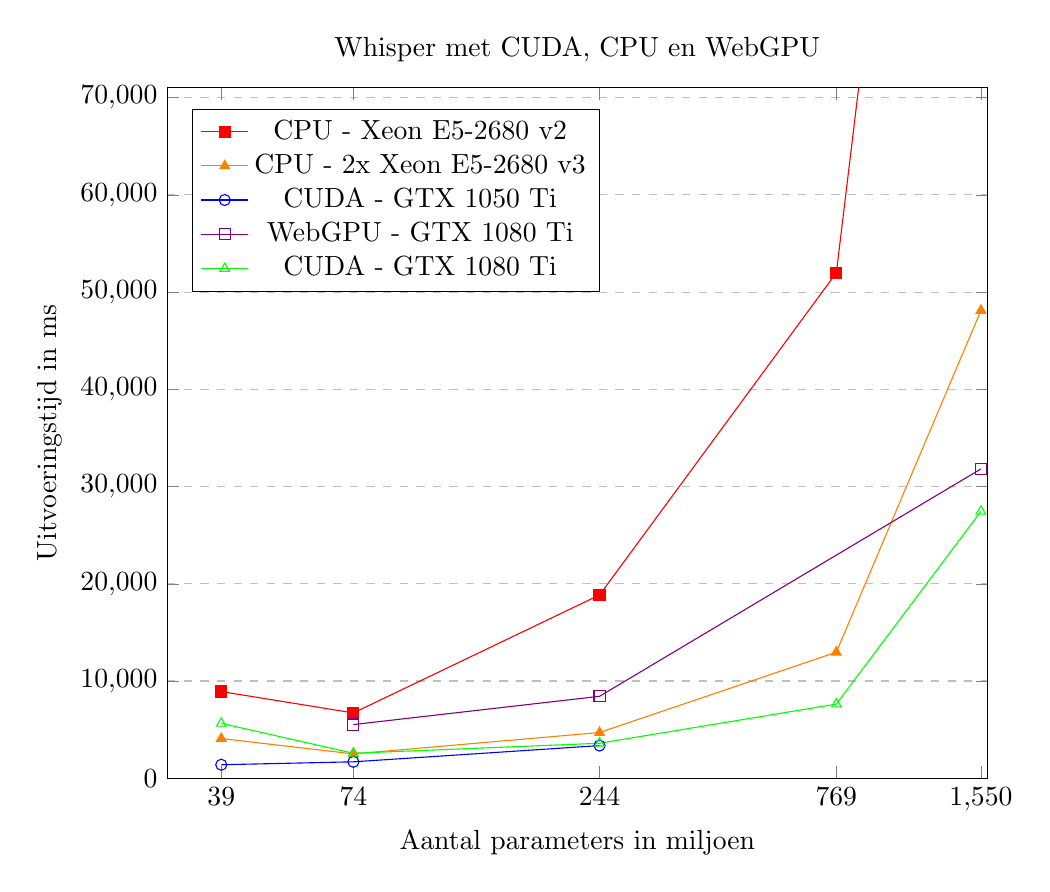
\begin{tikzpicture}
    \begin{semilogxaxis}[
        title={Whisper met CUDA, CPU en WebGPU},
        xlabel={Aantal parameters in miljoen},
        ylabel={Uitvoeringstijd in ms},
        xmin=30, xmax=1600,
        ymin=0, ymax=71000,
        xtick={39, 74, 244, 769, 1550},
        legend pos=north west,
        ymajorgrids=true,
        grid style=dashed,
        yticklabel style={
            /pgf/number format/fixed,
        },
        scaled y ticks=false
    ]
    \addplot[
            color=red,
            mark=square*
        ]
        coordinates {(39,8919)(74,6721)(244,18849)(769,51980)(1550,175378)};
        \addlegendentry{CPU - Xeon E5-2680 v2}
    \addplot[
        color=orange,
        mark=triangle*
        ]
        coordinates {(39,4088)(74,2508)(244,4706)(769,12963)(1550,48107)};
        \addlegendentry{CPU - 2x Xeon E5-2680 v3}
    \addplot[
            color=blue,
            mark=o
        ]
        coordinates {(39,1393)(74,1694)(244,3362)};
        \addlegendentry{CUDA - GTX 1050 Ti}
    \addplot[
            color=violet,
            mark=square
        ]
        coordinates {(74,5526)(244,8431)(1550,31814)};
        \addlegendentry{WebGPU - GTX 1080 Ti}
    \addplot[
            color=green,
            mark=triangle
        ]
        coordinates {(39,5647)(74,2574)(244,3602)(769,7629)(1550,27448)};
        \addlegendentry{CUDA - GTX 1080 Ti}
    \end{semilogxaxis}
\end{tikzpicture}

% pip3 install torch torchvision==0.15.0 torchaudio==2.0.0 --index-url https://download.pytorch.org/whl/cu117
% pip3 install torch torchvision==0.15.0 torchaudio==2.0.0 --index-url https://download.pytorch.org/whl/cpu
% pip3 uninstall torch torchvision==0.15.0 torchaudio==2.0.0
% pip3 cache purge

\subsection*{Resultaten van de Whisper test}

Uit de resultaten kan worden afgeleid dat zelfs krachtige processoren zoals de Xeon E5-2680 v2 en v3 al snel niet op kunnen tegen de parallelle rekenkracht van grafische kaarten. De experimentele \textit{WebGPU} implementatie van \textcite{Fleetwood2024} kan niet evenaren aan de \textit{CUDA} implementatie deze verschillen gemiddeld 53,4\%, 57,2\% en 13,7\% bij de \textit{base}, \textit{small} en \textit{large} implementaties van Whisper respectievelijk. Relatief gezien ten opzichte van de processor prestaties van de \textit{Xeon E5-2680 v2} is dit geen groot verschil, omdat deze processor prestaties naarmate dat het Whisper model wordt uitgevoerd met toenemende parameter grootte niet goed schaalt. Het is wel belangrijk te vermelden dat bij de \textit{large} implementatie van Whisper het VRAM geheugen gebruik van het model substantieel lager was in \textit{WebGPU} dan in de \textit{CUDA} implementatie en dat hierdoor het model mogelijks een andere kwantisering wordt toegepast. Dit kan leiden tot een verlaagd VRAM gebruik.

\bigbreak{}

Initieel presteren de twee \textit{Xeon E5-2680 v3} processoren beter dan de \textit{WebGPU} implementatie. Maar naarmate het model in parameter grootte toeneemt wordt duidelijk dat de uitvoeringstijd sterk begint te stijgen. De verhoogde parallelle rekenkracht van de grafische kaarten zijn hiervoor beter opgewassen. Ook speelt de verhoogde \textit{VRAM} bandbreedte hier een rol. 

\bigbreak{}

Omwille van het beperkte geheugen waarover de \textit{GTX 1050 Ti} beschikt (4GB) kon deze enkel worden getest tot en met het kleine \textit{Whisper} model (244 miljoen parameters). Dit is een belangrijke beperking om in acht te houden bij gebruiken grafische kaarten voor de uitvoering van AI-modellen. Omdat grafische kaarten in het algemeen over minder geheugen beschikken dan waarover een processor beschikt. Wanneer \textit{WebGPU} of \textit{CUDA} technologie wordt gebruikt om AI-modellen uit te voeren moet dus rekening worden gehouden hoeveel beschikbaar werkgeheugen er is. Wanneer deze grens wordt bereikt wordt vaak het gedeelde geheugen gebruikt, hierdoor wordt de bandbreedte sterk beperkt omdat er een constante uitwisseling moet plaats vinden tussen het geheugen van de grafische kaart en het standaard \textit{random access memory} van de processor.

\bigbreak{}

\begin{tabular}{ |p{6cm}|p{3cm}|p{3cm}|p{3cm}|  }
    \hline
    \multicolumn{4}{|c|}{\textit{Random Access Memory} snelheden} \\
    \hline
    Component& DDR generatie & Klokfrequentie & Bandbreedte \\
    \hline
        Xeon E5-2680 V2             & DDR 3     & 1866 MHz  & 59.7 GB/s \\
        2x Xeon E5-2680 V3          & DDR 4     & 2133 MHz  & 136 GB/s  \\
        Nvidia GeForce GTX 1050 Ti  & GDDR 5    & 7008 MHz  & 112.1 GB/s\\
        Nvidia GeForce GTX 1080 Ti  & GDDR 5X   & 11000 MHz & 484.4 GB/s\\
    \hline
\end{tabular}

\bigbreak{}

Deze gegevens werden verzameld op basis van de \textcite{Intel2013,Intel2014} specificaties voor de processoren en de \textcite{TechPowerUp2016, TechPowerUp2017} specificaties voor de grafische kaarten.

\section{wgpu-bench}

Om de performantie te testen van WebGPU werd wgpu-bench uitgevoerd.

Hiervoor werd rust geïnstalleerd, en gebruik gemaakt van Visual Studio Community 2022 in combinatie met Visual Studio Build-Tools 2022, waarbij de \textit{Desktop development with C++} module werd meegeïnstalleerd.

De broncode moest hierna gebouwd worden.

% rustup default nightly-x86_64-pc-windows-msvc

\break{}
